% Include at the figure's native 178 mm width. Do not scale labels below 10 pt.
% EPT indices refer to the interposed monitor, not to the outer Hyper-V.
\begin{figure*}[t]
  \centering
  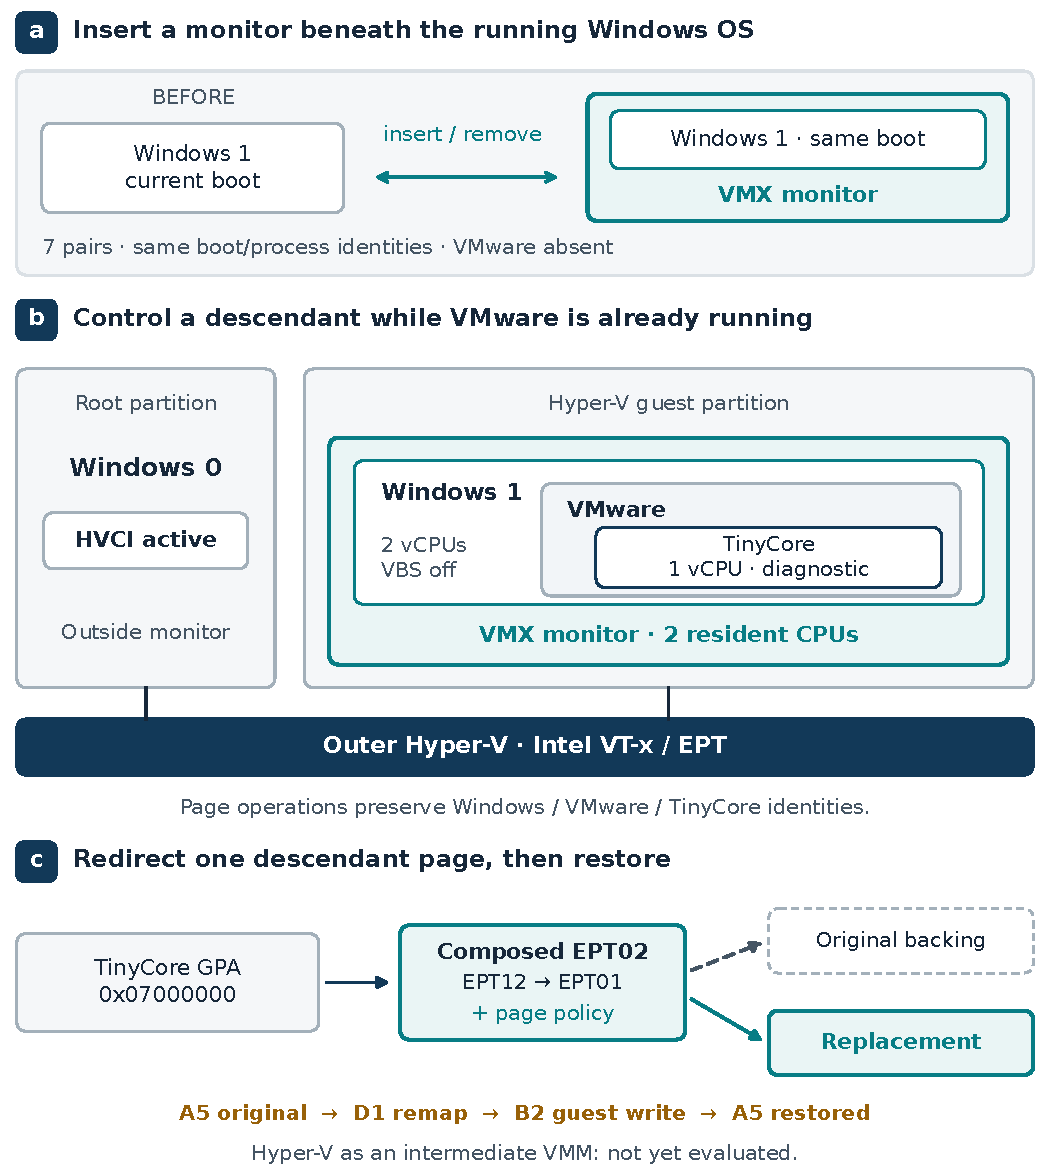
\includegraphics[width=178mm]{figures/architecture.pdf}
  \caption{Two separately evaluated experiments. (a) Windows 1 enters and
  leaves the monitor within one boot, without an intermediate VMM running.
  (b) VMware and TinyCore are already running during descendant-page operations;
  Windows 0 and HVCI remain in the outer Hyper-V root partition.
  (c) A policy overrides one composed leaf. The four-byte readback sequence
  covers the original, replacement, guest write, and restored original.
  Backing belongs to the monitor/Windows 1 physical-address domain.}
  \Description{Panel a shows the same Windows instance before and after a
  VMX monitor is inserted beneath it. Panel b shows sibling root and guest
  partitions above the outer Hyper-V. Only the guest partition contains the
  monitor, Windows 1, VMware, and TinyCore. Panel c branches the composed EPT
  translation of TinyCore GPA 0x07000000 toward original or replacement
  backing. A dashed arrow marks the normal or restored route; a solid arrow
  marks the replacement route. Readbacks progress from A5 to D1 to B2 and
  return to A5. A final note identifies intermediate Hyper-V testing as pending.}
  \label{fig:architecture}
\end{figure*}
